% ================================================================================
% E-AI Tutorial Slides
% Filename: lec17.tex
%
% Roland Potthast 2025/2026
% Licence: CC-BY4.0
% ================================================================================
\documentclass[aspectratio=169]{beamer}

% --- Load lecture macros --------------------------------------------------------
% =================================================================================
% E-AI Tutorial Tex Macros for Slides
% Filename: lec_macros.tex
% 
% DWD, Roland Potthast 2025/2026
% Licence: CC-BY4.0
% =================================================================================

% --------------------------------------------------------------------------------
% Packages
% --------------------------------------------------------------------------------
\usepackage[T1]{fontenc}
\usepackage{lmodern}
\usepackage{graphicx}
\usepackage{tikz}
\usepackage{ragged2e}
\usepackage{xcolor}
\usepackage{tcolorbox}
\tcbuselibrary{listings,skins,breakable}
\usepackage{listings}
\tcbuselibrary{breakable}
\usepackage{graphicx}
\usepackage{fancybox}
\usepackage{xcolor}
\usepackage{xparse}
\usepackage{tikz}
\usepackage{fontawesome5}
\usepackage{amsmath,amssymb}
\usepackage{hyperref}
\usepackage{adjustbox}
% in lec_macros.tex (or lec17.tex preamble)
\usetikzlibrary{calc}

% Shortcuts for number sets
\newcommand{\R}{\mathbb{R}}

\usetikzlibrary{positioning,arrows.meta}


% --------------------------------------------------------------------------------
% Beamer setup
% --------------------------------------------------------------------------------
\setbeamertemplate{navigation symbols}{}
\setbeamercolor{background canvas}{bg=white}
\usepackage{pifont}
\usepackage{xcolor}

\usepackage{pifont}
\newcommand{\mdcheck}{\textcolor{green!70!black}{\ding{51}}}

% --------------------------------------------------------------------------------
% Colours
% --------------------------------------------------------------------------------
\definecolor{DWDblue}{RGB}{0,68,136}
\setbeamercolor{DWDrule}{fg=DWDblue}
\definecolor{codegreen}{rgb}{0.0, 0.5, 0.0} % Dark green for comments
\definecolor{codeblue}{rgb}{0.0, 0.2, 0.6} % Muted dark blue for keywords
\definecolor{codered}{rgb}{0.6, 0.1, 0.1}  % Muted red for strings
\definecolor{codegray}{rgb}{0.4, 0.4, 0.4} % Gray for numbers and operators
\definecolor{backcolor}{rgb}{0.97, 0.97, 0.97} % Very light gray background
\definecolor{lightblue}{RGB}{220, 230, 241} % Light blue for alternating rows
\definecolor{headerblue}{RGB}{180, 200, 230} % Slightly darker blue for headers
\definecolor{appendixblue}{RGB}{200, 220, 240} % Blue for appendix header
\definecolor{darkgreen}{RGB}{0,110,80}

\newcommand{\y}[1]{%
\colorbox{yellow!50}{#1}%
}\newcommand{\g}[1]{%
\colorbox{darkgreen!30}{#1}%
}
\newcommand{\red}{\color{red}}

% --------------------------------------------------------------------------------
% 
% --------------------------------------------------------------------------------
\newcommand{\rtext}[1]{{\color{red}#1}}

\newenvironment{tightmath}{
  \setlength{\abovedisplayskip}{3pt}
  \setlength{\belowdisplayskip}{3pt}
  \setlength{\abovedisplayshortskip}{2pt}
  \setlength{\belowdisplayshortskip}{2pt}
}{}

% --------------------------------------------------------------------------------
% Fonts
% --------------------------------------------------------------------------------
\setbeamerfont{title}{size=\Large,series=\bfseries}
\setbeamerfont{normal text}{size=\normalsize}

% --------------------------------------------------------------------------------
% Slide metadata
% --------------------------------------------------------------------------------
\newcommand{\LectureAuthor}{Roland Potthast}
\newcommand{\LectureYear}{2025--2026}

% --------------------------------------------------
% Header with logos
% --------------------------------------------------
\newcommand{\toplogos}{
  \noindent
  \vspace*{-5mm}
  \begin{minipage}{\textwidth}
    \raisebox{-0.5\height}{\includegraphics[height=1cm]{../../images/img00/ecmwf.png}}
    \hfill
    \raisebox{-0.5\height}{\includegraphics[height=0.9cm]{../../images/img00/university-of-reading-logo-vector.png}}
    \hfill
    \raisebox{-0.5\height}{\includegraphics[height=0.7cm]{../../images/img00/DWD-Logo_2013.svg.png}}
  \end{minipage}

  \vspace{-1mm}
\noindent
\begin{tikzpicture}
  \draw[DWDblue, line width=0.6pt] (0,0) -- (\textwidth,0);
\end{tikzpicture}
  \vspace{-3mm}
}

% --------------------------------------------------
% Title macro
% --------------------------------------------------
\newcommand{\mytitle}[1]{%
  {\usebeamerfont{title}\normalsize\color{DWDblue} #1}%
  \vspace{2mm}
}

% --------------------------------------------------
% Two-column layout macro
% --------------------------------------------------
\newcommand{\mycolumns}[2]{%
  \begin{columns}[T,totalwidth=\textwidth]
    \begin{column}{0.48\textwidth}
      \justifying
      #1
    \end{column}
    \begin{column}{0.48\textwidth}
      #2
    \end{column}
  \end{columns}
}

\makeatletter
% --------------------------------------------------------------------------------
% Footer: line + author | lecture | year | slide number
% --------------------------------------------------------------------------------
\setbeamertemplate{footline}{
  \leavevmode

% --- horizontal line above footer --------------------------------------------
\hbox to \paperwidth{%
  \hskip\beamer@leftmargin
  \begin{tikzpicture}
    \draw[DWDblue, line width=0.6pt]
      (0,0) --
      (\dimexpr\paperwidth-\beamer@leftmargin-\beamer@rightmargin\relax,0);
  \end{tikzpicture}
  \hskip\beamer@rightmargin
}

\vskip 0.6ex

  % --- footer content -----------------------------------------------------------
  \hbox to \paperwidth{%
    \hskip\beamer@leftmargin
    \begin{beamercolorbox}[
      wd=\dimexpr\paperwidth-\beamer@leftmargin-\beamer@rightmargin\relax,
      ht=2.2ex,
      dp=1.0ex,
      leftskip=0pt,
      rightskip=0pt
    ]{author in head/foot}
      \tiny\color{DWDblue}
      \LectureAuthor \hfill \LectureNumber \hfill \LectureYear \hfill Slide \insertframenumber
    \end{beamercolorbox}
    \hskip\beamer@rightmargin
  }
  \vskip 0.8ex
}
\makeatother

% ================================================================================
% Environment for Slides
% Arguments:
%   #1 : title
%   #2 : left column content
%   #3 : right column content
% ================================================================================
\newenvironment{myslide}[3]
{
  \begin{frame}[fragile]
    \toplogos
    \mytitle{#1}
    \begin{columns}[T,totalwidth=\textwidth]
      \begin{column}{0.48\textwidth}
        #2
      \end{column}
      \begin{column}{0.48\textwidth}
        #3
      \end{column}
    \end{columns}
  \end{frame}
}
{}

% Define the Python syntax highlighting style
\lstdefinestyle{pythonstyle}{
    language=Python,
    basicstyle=\ttfamily\small,    % Monospace font
    keywordstyle=\color{codeblue}\bfseries, % Keywords in blue
    stringstyle=\color{codered},  % Strings in red
    commentstyle=\color{codegreen}\itshape, % Comments in green italics
    numberstyle=\tiny\color{codegray}, % Line numbers in gray
    backgroundcolor=\color{gray!5}, % Light gray background
    breaklines=true,
    columns=fixed,
    showspaces=false,
    showstringspaces=false,
    keepspaces=true,
    numbers=left, % Show line numbers
    numbersep=5pt, % Adjust separation between numbers and text
    xleftmargin=7pt, % **Fix: Keeps numbers inside the box**
    framexleftmargin=15pt, % **Fix: Adds padding inside the box for numbers**
}


% ================================================================================
% Listing Environment
% ================================================================================
\newtcblisting{codeonly}[2][]{%
  listing only,
  listing options={
		style=pythonstyle, 
		basicstyle=\ttfamily\fontsize{9pt}{12pt}\selectfont,
		tabsize=2,          % Tabs = 2 spaces
    showtabs=false      % Don't show visible tab markers
		},
  breakable,
  colback=gray!5,
  colframe=gray!30,
  boxrule=0.2pt,
  arc=1.5mm,
  left=2mm, right=2mm, top=-2mm, bottom=-1mm,
  before skip=2pt, after skip=2pt,
  coltitle=gray!100,
  title={#2},
  fonttitle=\bfseries\footnotesize,
  #1
}

\makeatletter
\setbeamertemplate{headline}{
  \leavevmode
  \vspace*{2mm}
  \hbox to \paperwidth{%
    \hskip\beamer@leftmargin
    \begin{minipage}{\dimexpr\paperwidth-\beamer@leftmargin-\beamer@rightmargin\relax}
      \raisebox{-0.5\height}{%
        \includegraphics[height=1cm]{../../images/img00/ecmwf.png}%
      }\hfill
      \raisebox{-0.5\height}{%
        \includegraphics[height=0.9cm]{../../images/img00/university-of-reading-logo-vector.png}%
      }\hfill
      \raisebox{-0.5\height}{%
        \includegraphics[height=0.7cm]{../../images/img00/DWD-Logo_2013.svg.png}%
      }
    \end{minipage}
    \hskip\beamer@rightmargin
  }

  \vspace{-2.5mm}

  \hbox to \paperwidth{%
    \hskip\beamer@leftmargin
    \begin{tikzpicture}
      \draw[DWDblue, line width=0.6pt]
        (0,0) --
        (\dimexpr\paperwidth-\beamer@leftmargin-\beamer@rightmargin\relax,0);
    \end{tikzpicture}
    \hskip\beamer@rightmargin
  }

  \vspace{0mm}
}
\makeatother

\lstset{
  basicstyle=\ttfamily\footnotesize,
  columns=fullflexible,
  keepspaces=true,
  showstringspaces=false,
  upquote=true
}

% --------------------------------------------------------------------------------
% Image box with soft shadow (no fixed size)
% --------------------------------------------------------------------------------
\newcommand{\slideimage}[2][]{%
  \tcbox[
    colback=white,
    boxrule=0pt,
    arc=2mm,
    shadow={1mm}{-1mm}{0mm}{black!30},
    enhanced,
    left=0pt,
    right=0pt,
    top=0pt,
    bottom=0pt,
  ]{%
    \includegraphics[#1]{#2}%
  }%
}

% ------------------------------------------------------------
% Red rounded box overlay on an image
% Usage:
% \imgwithbox{<includegraphics>}{<x1>}{<y1>}{<x2>}{<y2>}
%
% Coordinates are in the same unit as you provide, typically cm.
% Lower-left corner (x1,y1), upper-right corner (x2,y2).
% ------------------------------------------------------------
\newcommand{\imgwithbox}[5]{%
\begin{tikzpicture}
  \node[anchor=south west, inner sep=0] (img) {#1};
  \begin{scope}[x={(img.south east)}, y={(img.north west)}]
    % coordinates are now normalized 0..1 of image width/height
    \draw[red, very thick, rounded corners=4pt]
      (#2,#3) rectangle (#4,#5);
  \end{scope}
\end{tikzpicture}%
}


% ============================================================
% Agenda highlight box from lecture number (1..20)
% 5 columns × 4 rows (20 lectures)
%
% User defines ONE rectangle region on the agenda image:
%   x in [\AgendaXLeft, \AgendaXRight]
%   y in [\AgendaYBottom, \AgendaYTop]
%
% Mapping:
%   row = mod(L-1,4) + 1    (top to bottom)
%   col = floor((L-1)/4)+1  (left to right)
%
% Box size inside each cell:
%   dx, dy ∈ (0..1]  fraction of cell width/height
%   (can be tuned per lecture)
%
% Outputs:
%   \AgBoxXone, \AgBoxYone, \AgBoxXtwo, \AgBoxYtwo
% ============================================================

% ------------------------------------------------------------
% REGION (you adjust these by trial & error)
% ------------------------------------------------------------
\def\AgendaXLeft{0.13}
\def\AgendaXRight{0.98}

\def\AgendaYTop{0.87}
\def\AgendaYBottom{0.03}

% ------------------------------------------------------------
% DEFAULT box size inside each cell (fractions of cell size)
% ------------------------------------------------------------
\def\AgendaBoxDX{1.05}   % 90% of cell width
\def\AgendaBoxDY{1.00}   % 80% of cell height

% ------------------------------------------------------------
% OUTPUT variables (used by your drawing overlay)
% ------------------------------------------------------------
\def\AgBoxXone{0.10}
\def\AgBoxYone{0.10}
\def\AgBoxXtwo{0.20}
\def\AgBoxYtwo{0.20}

% ------------------------------------------------------------
% MAIN FUNCTION
% Usage:
%   \setagendaboxforlecture{L}
%   \setagendaboxforlecture[dx][dy]{L}
%
% Example:
%   \setagendaboxforlecture{17}
%   \setagendaboxforlecture[0.75][0.60]{17}
% ------------------------------------------------------------
\NewDocumentCommand{\setagendaboxforlecture}{ O{\AgendaBoxDX} O{\AgendaBoxDY} m }{%
  \pgfmathtruncatemacro{\L}{#3}%

  % row/col mapping
  \pgfmathtruncatemacro{\row}{mod(\L-1,4)+1}% 1..4
  \pgfmathtruncatemacro{\col}{floor((\L-1)/4)+1}% 1..5

  % cell size
  \pgfmathsetmacro{\W}{(\AgendaXRight-\AgendaXLeft)/5.0}%
  \pgfmathsetmacro{\H}{(\AgendaYTop-\AgendaYBottom)/4.0}%

  % cell bounds
  \pgfmathsetmacro{\xAcell}{\AgendaXLeft + (\col-1)*\W}%
  \pgfmathsetmacro{\xBcell}{\AgendaXLeft + (\col)*\W}%

  % row=1 is top
  \pgfmathsetmacro{\yTopCell}{\AgendaYTop - (\row-1)*\H}%
  \pgfmathsetmacro{\yBotCell}{\AgendaYTop - (\row)*\H}%

  % box fractions dx,dy
  \pgfmathsetmacro{\dx}{#1}%
  \pgfmathsetmacro{\dy}{#2}%

  % mid point of the cell
  \pgfmathsetmacro{\xMid}{0.5*(\xAcell+\xBcell)}%
  \pgfmathsetmacro{\yMid}{0.5*(\yTopCell+\yBotCell)}%

  % half box size in absolute figure coordinates
  \pgfmathsetmacro{\xHalf}{0.5*\dx*\W}%
  \pgfmathsetmacro{\yHalf}{0.5*\dy*\H}%

  % export corners
  \xdef\AgBoxXone{\xMid-\xHalf}%
  \xdef\AgBoxXtwo{\xMid+\xHalf}%
  \xdef\AgBoxYone{\yMid-\yHalf}%
  \xdef\AgBoxYtwo{\yMid+\yHalf}%
}


\newcommand{\LectureNumber}{Lecture 17}

% --- Document -------------------------------------------------------------------
\begin{document}

% somewhere before the frame (or in lec17.tex)
% put this before the image
\setagendaboxforlecture{17}

% ================================================================================
% Slide
% ================================================================================
\begin{frame}[t,fragile, noframenumbering]

% --- Title ---------------------------------------------------------------------
\mytitle{Python and AI/ML for Weather, Climate and Environmental Applications}

% --- Content -------------------------------------------------------------------
\begin{columns}[T,totalwidth=\textwidth]

% --- Left column ---------------------------------------------------------------
\begin{column}[T]{0.34\textwidth}

\includegraphics[width=4.3cm]{../../images/img00/e-ai_illustration01.png}

\vspace{-2mm}
\begin{flushright}
\Large
Let us enjoy {\color{red!80}\faRocket} \\[0.3em]
playing {\color{yellow!90}\faRobot} with \\[0.3em]
Python {\color{green!70!black}\faPython} and AI/ML!\\
{\color{purple!80}\faBrain}\quad
{\color{blue!70}\faCogs}\quad

\end{flushright}

\end{column}

% --- Right column --------------------------------------------------------------
\begin{column}[T]{0.62\textwidth}

\vspace{-3mm}
\imgwithbox{\includegraphics[width=\linewidth]{../../images/img00/agenda.png}}
          {\AgBoxXone}{\AgBoxYone}{\AgBoxXtwo}{\AgBoxYtwo}

% --- End Columns, Column and Frame ---------------------------------------------
\end{column}
\end{columns}
\end{frame}


%!TEX root = lec17.tex
% ================================================================================
% Lecture 17 — Slide 01
% ================================================================================
\begin{frame}[t]

\mytitle{Why Emulators in Numerical Weather Prediction?}

\begin{columns}[T,totalwidth=\textwidth]

% ------------------------------------------------------------
\begin{column}[T]{0.5\textwidth}

\vspace{-2mm}
\includegraphics[width=6cm]{../../images/img17/nwp.png}

\footnotesize
\begin{itemize}
  \item High-resolution NWP is \\ \y{computationally expensive}
  \item Many applications do not require \\ full physical fidelity
  \item Fast forecasts enable \y{new applications} \\ and scale
\end{itemize}
\end{column}

% ------------------------------------------------------------
\begin{column}[T]{0.48\textwidth}
\footnotesize

\vspace{-2mm}
\textbf{Emulator concept}

\begin{itemize}
  \item Learns the forecast step: state $\rightarrow$ state
  \item Operates within an existing NWP ecosystem
  \item Preserves grids, variables, and semantics
\end{itemize}

\vspace{2mm}
\textbf{Goal of this lecture}

\begin{itemize}
  \item Understand emulator-based AI systems
  \item Compare AIFS and AICON
  \item Walk through AICON step by step
\end{itemize}

\vspace{2mm}
\footnotesize
\rtext{\bf Emulators complement numerical models — they do not replace physical understanding.}

\end{column}

\end{columns}



\end{frame}

%!TEX root = lec17.tex
% ================================================================================
% Lecture 17 — Slide 02
% ================================================================================
\begin{frame}[t,fragile]

\mytitle{Big-Tech AI Weather Models: Architectural Landscape}

\begin{columns}[T,totalwidth=\textwidth]

% ------------------------------------------------------------
\begin{column}[T]{0.48\textwidth}
\footnotesize

\textbf{GraphCast (Google DeepMind)}

\begin{itemize}
  \item \y{Graph Neural Network (GNN)}
  \item Icosahedral grid, $\sim$0.25$^\circ$
  \item Multi-mesh message passing
  \item Deterministic medium-range forecasts
\end{itemize}

\vspace{4mm}
\textbf{GenCast (Google DeepMind)}

\begin{itemize}
  \item \y{Diffusion model on graphs}
  \item Icosahedral grid, $\sim$1$^\circ$–0.25$^\circ$
  \item Probabilistic forecasting
  \item Explicit uncertainty representation
\end{itemize}



\end{column}

% ------------------------------------------------------------
\begin{column}[T]{0.48\textwidth}
\footnotesize

\textbf{Pangu-Weather (Huawei)}

\begin{itemize}
  \item \y{3D Transformer architecture}
  \item Regular lat--lon grid, $\sim$0.25$^\circ$
  \item Attention over space and vertical levels
  \item Image-like representation of atmosphere
\end{itemize}

\vspace{4mm}
\textbf{FourCastNet (NVIDIA)}

\begin{itemize}
  \item \y{Fourier Neural Operator (FNO)}
  \item Regular lat--lon grid, $\sim$0.25$^\circ$
  \item Spectral convolution in Fourier space
  \item Extremely fast inference
\end{itemize}

\end{column}

\end{columns}

\vspace{2mm}
\footnotesize
\rtext{\bf All models replace the forecast step — none are embedded in classical NWP systems.}

\end{frame}

%!TEX root = lec17.tex
% ================================================================================
% Lecture 17 — Slide 03
% ================================================================================
\begin{frame}[t,fragile]

\mytitle{Research and Operational AI Weather Systems}

\begin{columns}[T,totalwidth=\textwidth]

% ------------------------------------------------------------
\begin{column}[T]{0.48\textwidth}
\footnotesize

\textbf{Aurora (Microsoft)}

\begin{itemize}
  \item \y{Transformer-based foundation model}
  \item Regular lat--lon grids
  \item Multi-task Earth-system scope
  \item Research-driven, not NWP-native
\end{itemize}

\textbf{AIFS (ECMWF)}

\begin{itemize}
  \item Graph Neural Network (Anemoi)
  \item \y{ECMWF Flagship ML Model}
  \item Trained on ECMWF reanalysis ERA
  \item Operational global forecast system
\end{itemize}

\end{column}

% ------------------------------------------------------------
\begin{column}[T]{0.48\textwidth}
\footnotesize

\textbf{BRIS (Met Norway)}

\begin{itemize}
  \item Anemoi-based national system
  \item \y{Nested Grid Approach, high resolution}
  \item Independent training, AIFS-aligned
  \item Operational national usage
\end{itemize}

\textbf{AICON (DWD)}

\begin{itemize}
  \item Graph Neural Network (Anemoi)
  \item Native ICON triangular grid
  \item Trained on \y{ICON-DREAM reanalysis}
  \item Operational ICON emulator
\end{itemize}

\end{column}

\end{columns}

\vspace{4mm}
\footnotesize
\rtext{\bf European Meteorological Infrastructure is carrying out exciting development.}

\end{frame}

%!TEX root = lec17.tex
% ================================================================================
% Lecture 17 — Slide 04
% ================================================================================
\begin{frame}[t]

\mytitle{Anemoi based Emulators: Fields and Grids}

\begin{columns}[T,totalwidth=\textwidth]

% ------------------------------------------------------------
\begin{column}[T]{0.48\textwidth}
\centering
\footnotesize

\vspace{-4mm}
\includegraphics[width=\textwidth]{../../images/img17/AICON.png}

\end{column}

% ------------------------------------------------------------
\begin{column}[T]{0.48\textwidth}
\centering
\footnotesize
\textbf{Icosahedral Grid Representation}

\vspace{2mm}
\includegraphics[width=\textwidth]{../../images/img17/aicon_grid1.png}

\vspace{1mm}
Triangular ICON mesh used as the computational graph
for message passing and inference.

\end{column}

\end{columns}

\footnotesize
\rtext{\bf AICON learns a mapping on the ICON mesh, not on a Cartesian grid.}

\end{frame}

%!TEX root = lec17.tex
% ================================================================================
% Lecture 17 — Slide 05
% ================================================================================
\begin{frame}[t]
\mytitle{ICON-DREAM Reanalysis: High-quality training basis for AI emulators}

\begin{columns}[T,totalwidth=\textwidth]
% ------------------------------------------------------------
\begin{column}[T]{0.52\textwidth}
\vspace{-1mm}
\footnotesize

\textbf{Motivation}
\begin{itemize}
\item reanalyses are key for \y{climate services} and many applications
\item now also essential as \y{training basis} for AI-based NWP emulators
\end{itemize}

\vspace{0mm}
\textbf{ICON reanalysis framework at DWD}
\begin{itemize}
\item \textbf{ICON-DREAM:} global-to-regional \y{ensemble reanalysis}
\item \textbf{ICON-FORCE:} 2.1\,km ensemble reanalysis for Central Europe
\item focus on \y{Europe} and on \y{continuous updates} (2010--present)
\end{itemize}

\vspace{0mm}
ICON-DREAM delivers \y{consistent, high-resolution} data
\end{column}

% ------------------------------------------------------------
\begin{column}[T]{0.46\textwidth}
\vspace{-1mm}
\footnotesize

\textbf{ICON-DREAM: key characteristics}
\begin{itemize}
\item global ICON at \textbf{13\,km}, 120 levels
\item two-way nest over Europe at \textbf{6.5\,km}
\item DA: \y{LETKF} with \textbf{20-member ensemble} for $B$-covariances
\item ensemble at 40\,km (20\,km over Europe)
\end{itemize}

\vspace{2mm}
\textbf{ICON-FORCE (2\,km):}
\begin{itemize}
\item hourly LETKF (KENDA), incl.\ radar + SEVIRI
\item 2-moment microphysics, snow / SST analyses
\end{itemize}

\vspace{1mm}
\textbf{Outlook:}
backward extension to the 1980s using rescued obs + CDR products.
\end{column}
\end{columns}

\end{frame}




%!TEX root = lec17.tex
% ================================================================================
% Lecture 17 — Slide 05
% ================================================================================
\begin{frame}[t,fragile]

\mytitle{AICON Walkthrough: Environment Setup}

\vspace{-1mm}
\centering
{\color{blue}\bf Thanks to {\sl Florian Prill} for a great Notebook!}

\begin{columns}[T,totalwidth=\textwidth]

% ------------------------------------------------------------
\begin{column}[T]{0.48\textwidth}
\footnotesize

\textbf{Core ML stack}

\begin{itemize}
  \item Python $\ge$ 3.10
  \item PyTorch (CPU or CUDA)
  \item PyTorch Lightning
  \item PyTorch Geometric (PyG)
\end{itemize}

\textbf{Anemoi framework}

\begin{itemize}
  \item \texttt{anemoi-core} (graphs, models, training)
  \item \texttt{anemoi-datasets} (Zarr + YAML I/O)
  \item \texttt{anemoi-inference} (generic inference)
  \item Supporting packages (e.g. transforms)
\end{itemize}

\end{column}

% ------------------------------------------------------------
\begin{column}[T]{0.48\textwidth}
\footnotesize

\textbf{Data and configuration}

\begin{itemize}
  \item Zarr (chunked training data)
  \item Xarray (inspection and analysis)
  \item eccodes + earthkit (GRIB2 handling)
  \item Hydra / OmegaConf (YAML configuration)
\end{itemize}

\textbf{Recommended setup}

\begin{itemize}
  \item Pinned \texttt{requirements.txt}
  \item Virtual environment or container
  \item Consistent library versions
\end{itemize}

\end{column}

\end{columns}

\vspace{4mm}
\footnotesize
\rtext{\bf Reproducibility depends on a stable, fully controlled software environment.}

\end{frame}

%!TEX root = lec17.tex
% ================================================================================
% Lecture 17 — Slide 07
% ================================================================================
\begin{frame}[t,fragile]

\mytitle{AICON Walkthrough: Manual Setup (Packages and ecCodes)}

\begin{columns}[T,totalwidth=\textwidth]

% ------------------------------------------------------------
\begin{column}[T]{0.42\textwidth}
\footnotesize

\vspace{-2mm}
\textbf{Install required Python packages}

\begin{codeonly}{Pinned Python environment}
# Install all required packages (version!)
%pip install --no-cache-dir -U -r ../requirements.txt

# Inspect installed versions
!pip freeze
\end{codeonly}

\vspace{1mm}
Exact package versions are critical for
PyTorch, PyG, Lightning, and Anemoi compatibility.

\end{column}

% ------------------------------------------------------------
\begin{column}[T]{0.56\textwidth}
\footnotesize

\vspace{-2mm}
\textbf{Configure ecCodes definitions}

\begin{minipage}{6cm}
\begin{lstlisting}
import os
from pathlib import Path

# Path to ICON/DWD ecCodes definitions
# (provided with the repo)
edzw_defs = Path("eccodes/definitions.edzw").resolve()

# Standard ecCodes definitions (system install)
std_defs = "/path/to/eccodes/definitions"

os.environ["ECCODES_DEFINITION_PATH"] = \
    f"{edzw_defs}:{std_defs}"
\end{lstlisting}
\end{minipage}

\vspace{1mm}
\color{darkgreen}
ICON GRIB decoding requires extended
definition tables beyond standard ecCodes.

\end{column}

\end{columns}


\end{frame}

%!TEX root = lec17.tex
% ================================================================================
% Lecture 17 — Slide 08
% ================================================================================
\begin{frame}[t,fragile]

\mytitle{AICON Walkthrough: Notebook Initialization}

\begin{columns}[T,totalwidth=\textwidth]

% ------------------------------------------------------------
\begin{column}[T]{0.48\textwidth}
\footnotesize

\textbf{Jupyter and runtime setup}

\begin{codeonly}{Notebook basics}
% Enable autoreload for iterative development
%load_ext autoreload
%autoreload 2

# Standard imports
import os
import numpy as np
import torch
\end{codeonly}

\vspace{1mm}
Ensures code changes are picked up
and the runtime environment is visible.

\end{column}

% ------------------------------------------------------------
\begin{column}[T]{0.51\textwidth}
\footnotesize

\textbf{Determinism and sanity checks}

\begin{codeonly}{Reproducibility checks}
# Fix random seeds
torch.manual_seed(42)
np.random.seed(42)

# Check PyTorch device
device = torch.device("cuda" if torch.cuda.is_available() else "cpu")
print("Using device:", device)
\end{codeonly}

\vspace{1mm}
Deterministic behavior is essential
for debugging and scientific comparison.

\end{column}

\end{columns}

\footnotesize
\rtext{\bf Initialization is not boilerplate — it defines the experimental contract.}

\end{frame}

% ================================================================================
% Lecture 17 — Slide 09
% ================================================================================
\begin{frame}[t,fragile]
\mytitle{AICON training setup (Anemoi): config-driven workflow}

\begin{columns}[T,totalwidth=\textwidth]
% ------------------------------------------------------------
\begin{column}[T]{0.48\textwidth}
\vspace{-1mm}
\footnotesize

\textbf{Main idea}
\begin{itemize}
\item training is \y{fully controlled by YAML configs}
\item Hydra composes config blocks:
\begin{itemize}
\item data (Zarr), variables, normalization
\item model architecture (AICON / GNN)
\item trainer settings (epochs, batch, strategy)
\end{itemize}
\end{itemize}

\vspace{-2mm}
\textbf{Workflow}
\begin{itemize}
\item choose config (start from \y{integration test})
\item instantiate trainer
\item run training (checkpoints + logger)
\end{itemize}

\end{column}

% ------------------------------------------------------------
\begin{column}[T]{0.48\textwidth}
\vspace{-1mm}
\footnotesize

\textbf{Notebook pattern (core lines)}
\begin{lstlisting}
config_filename = "test_aicon_01.yaml"

# Hydra loads and resolves config
config = load_config(config_filename)

# Anemoi trainer wraps Lightning
trainer = AnemoiTrainer(config)

# run training
trainer.train()
\end{lstlisting}

\vspace{1mm}
\textbf{Outputs}

\vspace{-2mm}
\begin{itemize}
\item checkpoints: \texttt{last.ckpt}, \texttt{inference-last.ckpt}
\item logs: TensorBoard / MLflow-style metrics
\end{itemize}

\end{column}
\end{columns}

\end{frame}

% ================================================================================
% Lecture 17 — Slide 10
% ================================================================================
\begin{frame}[t]
\mytitle{Training diagnostics: loss curve and experiment logger}

\begin{columns}[T,totalwidth=\textwidth]
% ------------------------------------------------------------
\begin{column}[T]{0.40\textwidth}
\vspace{-1mm}
\footnotesize

\textbf{What we monitor}
\begin{itemize}
\item training loss vs epoch/step
\item validation loss (generalization)
\item learning rate schedule
\item walltime + throughput
\end{itemize}

\vspace{2mm}
\textbf{Why it matters}
\begin{itemize}
\item early detection of instability
\item reproducible experiments
\item compare model variants
\end{itemize}

\vspace{2mm}
\color{red}\bf
\textbf{Take-away:}
training is \y{observable} and \y{traceable}.
\end{column}

% ------------------------------------------------------------
\begin{column}[T]{0.60\textwidth}


\vspace{-5mm}
\begin{center}
% Replace with your actual images from the notebook / export
\includegraphics[width=0.6\linewidth]{../../images/img17/aicon_loss_curve.png}

\vspace{1mm}
\includegraphics[width=0.85\linewidth]{../../images/img17/aicon_logger.png}
\end{center}

\end{column}
\end{columns}

\end{frame}

% ================================================================================
% Lecture 17 — Slide 11
% ================================================================================
\begin{frame}[t]
\mytitle{AICON training workflow (overview)}

\vspace{-2mm}
\begin{center}
% Put your overview graphic exported from the notebook / created by you
\includegraphics[width=0.96\linewidth]{../../images/img17/anemoi_icon_overview.png}
\end{center}

\vspace{-2mm}
\footnotesize
\textbf{Pipeline:} ICON data $\rightarrow$ graph dataset $\rightarrow$ training config $\rightarrow$ trainer $\rightarrow$ checkpoints + logs
\end{frame}

% ================================================================================
% Lecture 17 — Slide 12
% ================================================================================
\begin{frame}[t,fragile]
\mytitle{Training configuration: input and outputs}

\begin{columns}[T,totalwidth=\textwidth]

% ------------------------------------------------------------
\begin{column}[T]{0.52\textwidth}
\vspace{-1mm}
\footnotesize
\textbf{Input data (from config)}
\vspace{1mm}

\begin{codeonly}{text}
ICON mesh (NetCDF):
  <.../icon_mesh.nc>

Training interval:
  <YYYY-MM-DD HH> ... <YYYY-MM-DD HH>

Data files:
  <...>  (joined list)
\end{codeonly}

\vspace{1mm}
\textbf{Key point:} a single config fixes both \y{data geometry} and \y{time range}.
\end{column}

% ------------------------------------------------------------
\begin{column}[T]{0.46\textwidth}
\vspace{-1mm}
\footnotesize
\textbf{Output directories}
\vspace{1mm}

\begin{codeonly}{text}
Checkpoints:
  <.../checkpoints/...>

Logs (incl. MLFlow):
  <.../logs/...>
\end{codeonly}

\vspace{2mm}
\color{red}\bf
\textbf{Take-away:}
config $\Rightarrow$ reproducible paths and artifacts.
\end{column}

\end{columns}
\end{frame}

% ================================================================================
% Lecture 17 — Slide 13
% ================================================================================
\begin{frame}[t]
\mytitle{Training dataset (Zarr) inspected as Xarray}

\vspace{-2mm}
\begin{columns}[T,totalwidth=\textwidth]

% ------------------------------------------------------------
\begin{column}[T]{0.36\textwidth}
\vspace{-1mm}
\footnotesize

\textbf{Key idea}
\begin{itemize}
\item dataset is a \y{4D tensor}:
\newline
(time, variable, ensemble, cell)
\item efficient I/O via \y{chunking} (Dask)
\item includes metadata:
\begin{itemize}
\item latitudes / longitudes
\item variable-wise statistics
(mean, std, min/max)
\end{itemize}
\end{itemize}

\vspace{1mm}
\color{red}\bf
\textbf{Take-away:}
this is \y{ML-ready} data with rich metadata.
\end{column}

% ------------------------------------------------------------
\begin{column}[T]{0.64\textwidth}
\vspace{-2mm}
\begin{center}
\includegraphics[width=\linewidth]{../../images/img17/dataset_xarray.png}
\end{center}
\end{column}

\end{columns}
\end{frame}

% ================================================================================
% Lecture 17 — Slide 14
% ================================================================================
\begin{frame}[t]
\mytitle{Vertical levels: selected ICON layers in the dataset}

\vspace{-2mm}
\begin{columns}[T,totalwidth=\textwidth]

% ------------------------------------------------------------
\begin{column}[T]{0.54\textwidth}
\vspace{-1mm}
\scriptsize

\textbf{Variables on model levels}
\vspace{1mm}

\begin{tabular}{lll}
\textbf{shortName} & \textbf{Name} & \textbf{Levels} \\
\hline
P  & Pressure                     & 49,57,64,70,75,79,86,...,120 \\
QV & Specific humidity            & 49,57,64,70,75,79,86,...,120 \\
T  & Temperature                  & 49,57,64,70,75,79,86,...,120 \\
U  & U-component of wind          & 49,57,64,70,75,79,86,...,120 \\
V  & V-component of wind          & 49,57,64,70,75,79,86,...,120 \\
W  & Vertical velocity (geom.)    & 49,57,64,70,75,79,86,...,120 \\
\hline
\end{tabular}

\vspace{4mm}
\footnotesize

\textbf{Forcings / static features (examples):}\\[2mm]
\scriptsize
EMIS\_RAD, FR\_LAND, FR\_LAKE, HSURF, Z0, insolation,
SSO\_*, sin/cos(latitude, longitude, local\_time, julian\_day)

\vspace{1mm}
\footnotesize
\textbf{Idea:} \y{multi-level state + forcings} $\Rightarrow$ complete ML input for AICON.
\end{column}

% ------------------------------------------------------------
\begin{column}[T]{0.46\textwidth}
\vspace{-2mm}
\raggedleft

% replace with your actual image path:
\includegraphics[width=0.8\linewidth]{../../images/img17/icon_levels.png}

\vspace{-2mm}
\footnotesize
\textbf{ICON level structure:} full model vertical grid (selection highlighted).
\end{column}

\end{columns}
\end{frame}

% ================================================================================
% Lecture 17 — Slide 15
% ================================================================================
\begin{frame}[t]
\mytitle{ICON multimesh: the hidden graph behind AICON}

\vspace{-2mm}
\begin{columns}[T,totalwidth=\textwidth]

% ------------------------------------------------------------
\begin{column}[T]{0.5\textwidth}
\vspace{-1mm}
\footnotesize

\textbf{Key idea}
\begin{itemize}
\item AICON does not run on a regular lat--lon grid
\item it uses ICON's \y{hierarchical triangular mesh}
\item the GNN operates on a \y{hidden multi-mesh}
\end{itemize}

\vspace{2mm}
\textbf{Multi-mesh principle}
\begin{itemize}
\item union of coarse-to-fine subgraphs \\
\quad R$n$B0 $\cup$ R$n$B1 $\cup$ ... $\cup$ R$n$Bk
\item mixes \y{short-range} + \y{long-range} edges
\item similar spirit as GraphCast multi-mesh
\end{itemize}

\vspace{2mm}
\color{red}\bf
\textbf{Take-away:}
the multi-mesh gives the GNN both \y{local physics} and \y{global context}.
\end{column}

% ------------------------------------------------------------
\begin{column}[T]{0.5\textwidth}
\vspace{-2mm}
\raggedleft
% Use the level-wise multimesh plot from the notebook:
\includegraphics[width=0.95\linewidth]{../../images/img17/grid_visual.png}

\vspace{4mm}
\scriptsize
Hidden mesh edges shown level-wise: coarse levels enable long-range interaction.
\end{column}

\end{columns}
\end{frame}

% ================================================================================
% Lecture 17 — Slide 16
% ================================================================================
\begin{frame}[t]
\mytitle{AICON model: encoder -- graph processor -- decoder}

\vspace{-2mm}
\begin{columns}[T,totalwidth=\textwidth]

% ------------------------------------------------------------
\begin{column}[T]{0.46\textwidth}
\vspace{-1mm}
\footnotesize

\textbf{Graph-to-graph forecasting}
\begin{itemize}
\item input: state + forcings on ICON cells (nodes)
\item output: next-step state (multi-var, multi-level)
\end{itemize}

\vspace{0mm}
\textbf{Architecture blocks}
\begin{itemize}
\item \textbf{Encoder:} maps raw variables to latent node/edge features
\item \textbf{Processor:} message passing on the mesh graph (several layers)
\item \textbf{Decoder:} projects latent features to physical output variables
\end{itemize}

\vspace{0mm}
\color{red}\bf
\textbf{Take-away:}
encoder/decoder makes the network \y{variable-agnostic} in latent space.
\end{column}

% ------------------------------------------------------------
\begin{column}[T]{0.54\textwidth}
\vspace{-2mm}
\raggedleft
% Use the architecture figure / screenshot from the notebook:
\includegraphics[width=0.9\linewidth]{../../images/img17/encoder_decoder.png}

\vspace{-2mm}
\scriptsize
Encoder maps physics variables $\rightarrow$ latent graph; decoder maps latent $\rightarrow$ output fields.
\end{column}

\end{columns}
\end{frame}

% ================================================================================
% Lecture 17 — Slide 17
% ================================================================================
\begin{frame}[t]
\mytitle{Graph structure: local neighborhoods on the ICON mesh}

\vspace{-2mm}
\begin{columns}[T,totalwidth=\textwidth]

% ------------------------------------------------------------
\begin{column}[T]{0.49\textwidth}
\vspace{-1mm}
\footnotesize

\textbf{Why this matters}
\begin{itemize}
\item AICON runs on the ICON grid as \y{graph neural network (GNN)}
\item each ICON cell $\Rightarrow$ one \y{graph node}
\item edges connect \y{mesh neighbors}
\end{itemize}

\vspace{2mm}
\textbf{Message passing view}
\begin{itemize}
\item prediction at one node uses information from:
\begin{itemize}
\item \textbf{1st neighbors} (directly connected)
\item \textbf{2nd neighbors} (neighbors-of-neighbors)
\end{itemize}
\item this defines the local receptive field of the GNN
\end{itemize}


\end{column}

% ------------------------------------------------------------
\begin{column}[T]{0.50\textwidth}
\vspace{-2mm}

\vspace{2mm}
\color{red}\bf
\textbf{Take-away:}
GNNs learn transport + interaction patterns through \y{local connectivity}.

\vspace{0mm}
\raggedleft
% Replace with your exported image:
\includegraphics[width=0.8\linewidth]{../../images/img17/graph_neighbours_crop.png}

\vspace{-2mm}
\scriptsize
Example: subgraph around one node (orange) with 1st and 2nd neighbors.
\end{column}

\end{columns}
\end{frame}

% ================================================================================
% Lecture 17 — Slide 18
% ================================================================================
\begin{frame}[t]
\mytitle{Graph Transformer attention: which neighbors matter?}

\vspace{-2mm}
\begin{columns}[T,totalwidth=\textwidth]

% ------------------------------------------------------------
\begin{column}[T]{0.48\textwidth}
\vspace{-1mm}
\footnotesize

\textbf{Graph Transformer vs.\ plain message passing}
\begin{itemize}
\item classic GNN: neighbors contribute via fixed averaging / sum
\item GraphTransformer: each edge gets a learned \y{attention weight}
\end{itemize}

\vspace{2mm}
\textbf{Interpretation}
\begin{itemize}
\item for one receiver node $i$, all incoming edges $(j \rightarrow i)$
\item attention weights $\alpha_{i,j}$ sum to 1 (per head)
\item thick edges $\Rightarrow$ \y{high influence} of neighbor $j$
\end{itemize}

\vspace{2mm}
\color{red}\bf
\textbf{Take-away:}
the model learns \y{where to look} on the graph depending on flow regime and structure.
\end{column}

% ------------------------------------------------------------
\begin{column}[T]{0.52\textwidth}
\vspace{-2mm}
\raggedleft

\includegraphics[width=0.86\linewidth]{../../images/img17/aicon_attention_graph.png}

\vspace{-1mm}
\includegraphics[width=0.86\linewidth]{../../images/img17/aicon_attention_graph2.png}

\vspace{-2mm}
\scriptsize
\textbf{Example:}
(top) ICON multi-mesh graph (coarse + fine connections);
(bottom) attention setup
\end{column}

\end{columns}
\end{frame}

% ================================================================================
% Lecture 17 — Slide 19
% ================================================================================
\begin{frame}[t, fragile]
\mytitle{Transfer learning: reuse weights on a finer hidden mesh}

\vspace{-2mm}
\begin{columns}[T,totalwidth=\textwidth]

% ------------------------------------------------------------
\begin{column}[T]{0.58\textwidth}
\vspace{-1mm}
\footnotesize

\textbf{Motivation}
\begin{itemize}
\item training on the finest multi-mesh is expensive
\item idea: \y{train on coarse mesh} and transfer to finer mesh
\end{itemize}

\vspace{2mm}
\textbf{What transfers well?}
\begin{itemize}
\item most encoder/processor/decoder weights
\item learned graph attention patterns are largely mesh-agnostic
\end{itemize}

\vspace{2mm}
\textbf{What must be adapted?}
\begin{itemize}
\item graph-dependent parameters:
\begin{itemize}
\item hidden node coordinates / embeddings
\item extra trainable node/edge attributes
\end{itemize}
\item these are re-initialized and fine-tuned on the new mesh
\end{itemize}

\vspace{2mm}
\color{red}\bf
\textbf{Take-away:}
efficient training strategy: \y{pretrain coarse} $\rightarrow$ \y{fine-tune fine}.
\end{column}

% ------------------------------------------------------------
\begin{column}[T]{0.4\textwidth}
\vspace{-1mm}
\footnotesize

\textbf{Example (AICON walkthrough)}
\begin{itemize}
\item change hidden mesh resolution:
\begin{itemize}
\item \texttt{max\_level\_multimesh: 3 $\rightarrow$ 4}
\end{itemize}
\item load weights only + enable transfer learning
\end{itemize}

\vspace{1mm}
\scriptsize
\begin{block}{Config idea (YAML)}
\begin{verbatim}
training:
  load_weights_only: true
  transfer_learning: true
  run_id: <pretrained_run_id>

graph:
  nodes:
    icon_mesh:
      node_builder:
        max_level_multimesh: 4
\end{verbatim}
\end{block}

\vspace{-1mm}
\footnotesize
This enables \y{cost-efficient scaling} to higher resolution.
\end{column}

\end{columns}
\end{frame}

% ================================================================================
% Lecture 17 — Slide 20
% ================================================================================
\begin{frame}[t]
\mytitle{Operational inference at DWD: why a dedicated tool?}

\begin{columns}[T,totalwidth=\textwidth]

% ------------------------------------------------------------
\begin{column}[T]{0.55\textwidth}
\vspace{-1mm}
\footnotesize

\textbf{Goal}
\begin{itemize}
\item run AICON forecasts \y{operationally} and \y{reproducibly}
\item integrate into existing NWP infrastructure (GRIB2, workflows, monitoring)
\end{itemize}

\vspace{2mm}
\textbf{Why not only \texttt{anemoi-inference}?}
\begin{itemize}
\item DWD-specific I/O and preprocessing (GRIB2 conventions)
\item additional input engineering (e.g.\ soil moisture index etc.)
\item packaging as stable runtime for ops (container)
\item hooks for monitoring and verification pipelines
\end{itemize}

\end{column}

% ------------------------------------------------------------
\begin{column}[T]{0.43\textwidth}
\vspace{-1mm}
\footnotesize

\textbf{Key ingredients}
\begin{itemize}
\item \textbf{checkpoint:} \texttt{inference-last.ckpt}
\item \textbf{input:} ICON / reanalysis data streams
\item \textbf{output:} GRIB2 forecast products
\end{itemize}

\vspace{2mm}
\textbf{Operational packaging}
\begin{itemize}
\item Apptainer / Singularity container
\item fixed paths to constants + weights
\item versioning: container + config + checkpoint
\end{itemize}

\vspace{2mm}
\color{red}\bf
\textbf{Take-away:}
DWD inference tool = \y{bridge from ML model to ops}.
\end{column}

\end{columns}
\end{frame}

% ================================================================================
% Lecture 17 — Slide 21
% ================================================================================
\begin{frame}[t]
\mytitle{Demo: AICON forecast from operational inference}

\vspace{-2mm}
\begin{center}
% Replace with your actual inference output figure
\includegraphics[width=0.96\linewidth]{../../images/img17/aicon_inference_forecast.png}
\end{center}

\vspace{-1mm}
\footnotesize
\textbf{Example product:} ML forecast fields generated from checkpoint + operational inference tool.
\end{frame}

% ================================================================================
% Slide 22 — FRAIM ecosystem graphic (Library + Apps + DAWID)
% ================================================================================
\begin{frame}[t, fragile]
\mytitle{FRAIM Ecosystem: Central Library, FRAIM-Apps, and DAWID Platform}

\centering
\vspace{0mm}

% requires:
% \usepackage{tikz}
% \usetikzlibrary{positioning,arrows.meta}

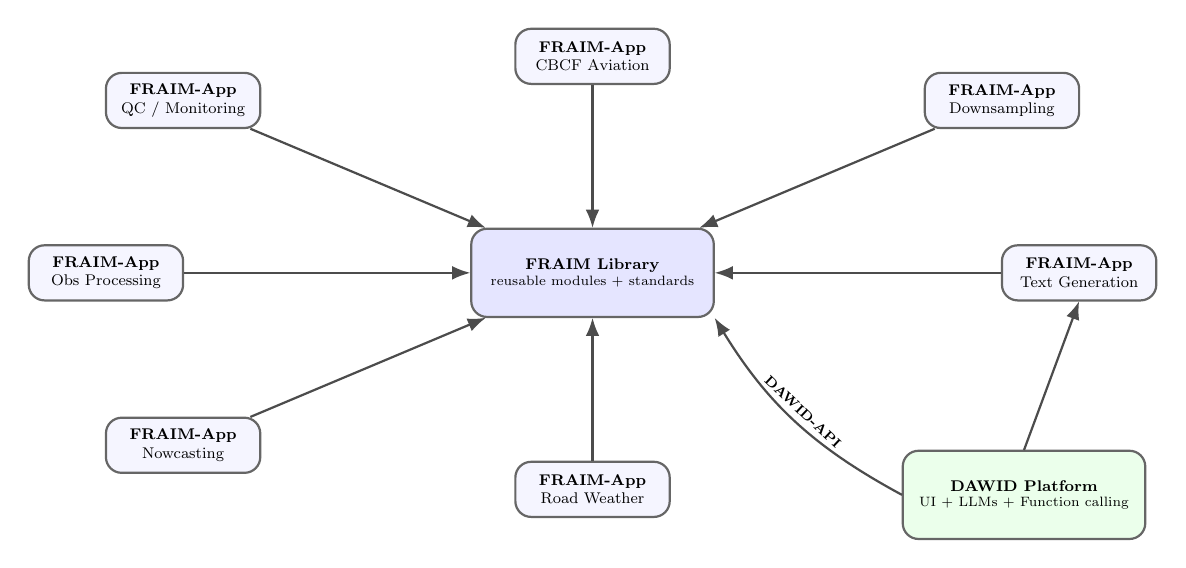
\begin{tikzpicture}[
  scale=0.7, transform shape,
  font=\footnotesize,
  >=Latex,
  node distance=12mm,
  box/.style={rounded corners=2mm, draw=black!60, thick, align=center, inner sep=2mm},
  app/.style={box, minimum width=28mm, minimum height=10mm, fill=blue!4},
  lib/.style={box, minimum width=44mm, minimum height=16mm, fill=blue!10},
  daw/.style={box, minimum width=44mm, minimum height=16mm, fill=green!8},
  arrow/.style={->, thick, draw=black!70}
]

% ------------------------------------------------------------
% Center: FRAIM library
% ------------------------------------------------------------
\node[lib] (lib) {\textbf{FRAIM Library}\\[-0.5mm]
\scriptsize reusable modules + standards};

% ------------------------------------------------------------
% FRAIM-Apps around (examples)
% ------------------------------------------------------------
\node[app, above left=18mm and 38mm of lib]  (app1) {\textbf{FRAIM-App}\\QC / Monitoring};
\node[app, above=26mm of lib]                (app2) {\textbf{FRAIM-App}\\CBCF Aviation};
\node[app, above right=18mm and 38mm of lib] (app3) {\textbf{FRAIM-App}\\Downsampling};
\node[app, right=52mm of lib]                (app4) {\textbf{FRAIM-App}\\Text Generation};
\node[app, below=26mm of lib]                (app6) {\textbf{FRAIM-App}\\Road Weather};
\node[app, below left=18mm and 38mm of lib]  (app7) {\textbf{FRAIM-App}\\Nowcasting};
\node[app, left=52mm of lib]                 (app8) {\textbf{FRAIM-App}\\Obs Processing};

% arrows from apps to library (reuse)
\draw[arrow] (app1) -- (lib);
\draw[arrow] (app2) -- (lib);
\draw[arrow] (app3) -- (lib);
\draw[arrow] (app4) -- (lib);
\draw[arrow] (app6) -- (lib);
\draw[arrow] (app7) -- (lib);
\draw[arrow] (app8) -- (lib);

% ------------------------------------------------------------
% DAWID Platform (placed bottom-right)
% ------------------------------------------------------------
\node[daw, below right=24mm and 34mm of lib] (dawid)
{\textbf{DAWID Platform}\\[-0.5mm]
\scriptsize UI + LLMs + Function calling};

% DAWID-API link to library
\draw[arrow] (dawid.west) to[bend left=15]
  node[midway, above, sloped, font=\scriptsize]{\textbf{DAWID-API}} (lib.south east);

% DAWID link to Postprocessing (rerouted to avoid Nowcasting area)
\draw[arrow] (dawid.north) -- (app4.south);

\end{tikzpicture}

\end{frame}

% ================================================================================
% Slide — Anemoi vs. FRAIM (1/3)
% ================================================================================
\begin{frame}[t]
\mytitle{Anemoi vs.\ FRAIM — What are they about?}

\begin{columns}[T,totalwidth=\textwidth]
% ------------------------------------------------------------
\begin{column}[T]{0.49\textwidth}
\footnotesize
\textbf{Anemoi (ECMWF \& Partners)}
\begin{itemize}
\item international collaboration to build \y{ML-based forecast models}
\item \textbf{end-to-end framework} for \y{training \& inference}
\item well-defined pipeline:
\newline
datasets $\rightarrow$ graphs/models $\rightarrow$ training $\rightarrow$ inference/deploy
\item \textbf{Open Source}, pan-European community
\end{itemize}

\vspace{2mm}
\textbf{Typical question:}
\newline
\emph{How do we train and operate an ML forecasting model operationally?}
\end{column}

% ------------------------------------------------------------
\begin{column}[T]{0.49\textwidth}

\vspace{-2mm}
\footnotesize
\textbf{FRAIM (E-AI / DWD / Partners)}
\begin{itemize}
\item international collaboration focused on \y{many AI applications}
\item \textbf{method toolbox / modular framework} across a broad portfolio:
\newline
products, services, and smaller AI components
\item platform/integration view:
\y{standards, building blocks, reuse}
\item \textbf{umbrella framework} (forecasting is only one use case)
\end{itemize}

\vspace{0mm}
\textbf{Typical question:}
\newline
\emph{How do we build a modular AI ecosystem for many meteorological products and services?}
\end{column}
\end{columns}
\end{frame}

% ================================================================================
% Slide — Anemoi vs. FRAIM (2/3)
% ================================================================================
\begin{frame}[t]
\mytitle{Pipeline view: where does each framework sit?}

\footnotesize
\vspace{-1mm}

\textbf{Anemoi:} lifecycle of an ML forecast model \\
\vspace{1mm}
\begin{center}
\begin{tabular}{c c c c c}
\textbf{Data} & $\rightarrow$ & \textbf{Training} & $\rightarrow$ & \textbf{Inference/Deploy} \\
(anemoi-datasets) & & (anemoi-training) & & (operational tooling) \\
\end{tabular}
\end{center}

\vspace{3mm}
\textbf{FRAIM:} system / toolbox view across multiple AI components \\
\vspace{1mm}
\begin{center}
\begin{tabular}{c c c c c}
\textbf{Use case} & $\rightarrow$ & \textbf{Modules} & $\rightarrow$ & \textbf{Integration/Operations} \\
Forecast / Nowcast / QC / \\
DA / Postproc
& &
training, surrogates, \\
QA, LLM, etc.
& &
platform + standards \\
\end{tabular}
\end{center}

\vspace{2mm}
\textbf{Take-away:}
\newline
Anemoi is \y{forecast-model-centric}, FRAIM is \y{architecture- \& reuse-centric}.
\end{frame}

% ================================================================================
% Slide — Anemoi vs. FRAIM (3/3)
% ================================================================================
\begin{frame}[t]

\mytitle{Concrete differences and a good integration story}

\begin{columns}[T,totalwidth=\textwidth]
% ------------------------------------------------------------
\begin{column}[T]{0.54\textwidth}

\vspace{0mm}
\footnotesize
\textbf{Differences (short \& concrete)}
\begin{itemize}
\item \textbf{Scope:}
Anemoi = end-to-end ML forecasting \\
FRAIM = modular AI toolbox for many meteorological products
\item \textbf{Core artifacts:}
\begin{itemize}
\item \textbf{Anemoi:} datasets, graphs, model weights, training pipelines
\item \textbf{FRAIM:} central library + reusable modules + standards
\end{itemize}
\item \textbf{Organization principle:}
\begin{itemize}
\item Anemoi: one coherent forecasting stack
\item FRAIM: many \y{use-case driven FRAIM-Apps} (each in its own repo)
\end{itemize}
\end{itemize}
\end{column}

% ------------------------------------------------------------
\begin{column}[T]{0.45\textwidth}

\vspace{-1mm}
\footnotesize
\textbf{How does this combine well?}
\begin{itemize}
\item FRAIM can \y{integrate} mfai or Anemoi as a forecasting or processing engine
\item FRAIM then provides:
\begin{itemize}
\item product-specific pipelines (QC, DA, verification, monitoring, etc.)
\item deployment patterns and operational standards
\end{itemize}
\end{itemize}

\vspace{2mm}
\color{red}\bf
\textbf{One-liner:}
\newline
Anemoi = \emph{forecast-model factory}; \\
FRAIM = \emph{modular product ecosystem}.
\end{column}
\end{columns}
\end{frame}

% ================================================================================
% Slide 26 — DAWID as LLM Platform and Integration Layer
% ================================================================================
\begin{frame}[t]
\mytitle{DAWID — LLM Platform, Tools, and FRAIM Integration}

\begin{columns}[T,totalwidth=\textwidth]

% ------------------------------------------------------------
\begin{column}[T]{0.53\textwidth}
\vspace{-1mm}
\footnotesize

\textbf{DAWID capabilities}
\begin{itemize}
\item \textbf{LLM user interface}
\begin{itemize}
\item chat + document context (RAG)
\item role-based workflows (science / dev / ops)
\end{itemize}

\item \textbf{Function calling}
\begin{itemize}
\item controlled execution of domain functions
\item structured I/O and provenance
\end{itemize}

\item \textbf{Agents (multi-step)}
\begin{itemize}
\item plan $\rightarrow$ call tools $\rightarrow$ validate
\end{itemize}
\end{itemize}

\vspace{1mm}
\textbf{Key idea:} DAWID is the \y{interactive AI cockpit}.
\end{column}


% ------------------------------------------------------------
\begin{column}[T]{0.46\textwidth}
\vspace{-1mm}
\footnotesize

\textbf{DAWID-API integration}
\begin{itemize}
\item \textbf{Unified API} to LLMs and tools
\begin{itemize}
\item multi-LLM backends
\item tool/function endpoints
\end{itemize}

\item \textbf{Link to FRAIM-Apps}
\begin{itemize}
\item FRAIM-App $\rightarrow$ DAWID-API: reasoning + tooling
\item consistent interface across products
\end{itemize}
\end{itemize}

\vspace{2mm}
\color{red}\bf
\textbf{Take-away:}
DAWID connects \y{LLMs + tools + FRAIM-Apps}.
\end{column}

\end{columns}
\end{frame}


% --- End Document ---------------------------------------------------------------
\end{document}
